% Q1V4: Rectangular Core with Two Series Air Gaps — Exam diagram (hybrid style C)
% Shows: core geometry, coil positions, gap locations, dimensions
% Strips: flux arrows, mu_r label, reluctance circuit (P-STACK-31)
\documentclass[border=10pt]{standalone}
\usepackage{tikz}
\usepackage{amsmath}
\usetikzlibrary{patterns, decorations.pathreplacing}
\renewcommand{\familydefault}{\sfdefault}

\begin{document}
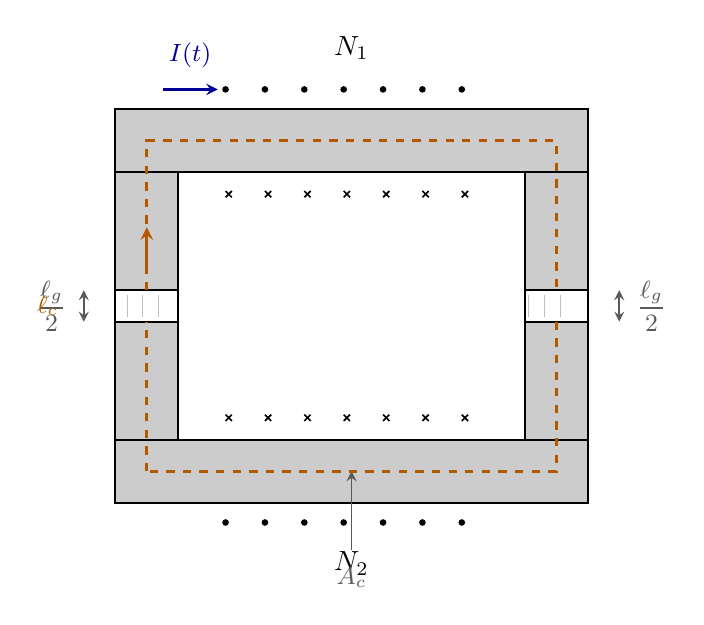
\begin{tikzpicture}[
    every node/.style={font=\sffamily},
    >=stealth,
    dim/.style={<->, line width=0.6pt, gray!70!black},
    dimlabel/.style={font=\sffamily\small, text=gray!70!black},
]

% === Rectangular core frame ===
\def\coreW{6}       % outer width
\def\coreH{5}       % outer height
\def\limbW{0.8}     % limb/yoke thickness
\def\gapH{0.4}      % each gap height (total = 2 * gapH = lg)

% Top yoke
\fill[gray!40, draw=black, line width=0.8pt]
    (0,{\coreH-\limbW}) rectangle (\coreW,\coreH);

% Bottom yoke
\fill[gray!40, draw=black, line width=0.8pt]
    (0,0) rectangle (\coreW,\limbW);

% Left limb — top half (above gap)
\fill[gray!40, draw=black, line width=0.8pt]
    (0,{0.5*\coreH+0.5*\gapH}) rectangle (\limbW,{\coreH-\limbW});
% Left limb — bottom half (below gap)
\fill[gray!40, draw=black, line width=0.8pt]
    (0,\limbW) rectangle (\limbW,{0.5*\coreH-0.5*\gapH});

% Right limb — top half (above gap)
\fill[gray!40, draw=black, line width=0.8pt]
    ({\coreW-\limbW},{0.5*\coreH+0.5*\gapH}) rectangle (\coreW,{\coreH-\limbW});
% Right limb — bottom half (below gap)
\fill[gray!40, draw=black, line width=0.8pt]
    ({\coreW-\limbW},\limbW) rectangle (\coreW,{0.5*\coreH-0.5*\gapH});

% === Air gap 1 (left limb) ===
\fill[white]
    (0,{0.5*\coreH-0.5*\gapH}) rectangle (\limbW,{0.5*\coreH+0.5*\gapH});
\draw[line width=0.8pt]
    (0,{0.5*\coreH-0.5*\gapH}) rectangle (\limbW,{0.5*\coreH+0.5*\gapH});
% Hatching
\foreach \xx in {0.15, 0.35, 0.55} {
    \draw[thin, gray!50]
        (\xx,{0.5*\coreH-0.35*\gapH}) -- (\xx,{0.5*\coreH+0.35*\gapH});
}

% === Air gap 2 (right limb) ===
\fill[white]
    ({\coreW-\limbW},{0.5*\coreH-0.5*\gapH}) rectangle (\coreW,{0.5*\coreH+0.5*\gapH});
\draw[line width=0.8pt]
    ({\coreW-\limbW},{0.5*\coreH-0.5*\gapH}) rectangle (\coreW,{0.5*\coreH+0.5*\gapH});
% Hatching
\foreach \xx in {5.25, 5.45, 5.65} {
    \draw[thin, gray!50]
        (\xx,{0.5*\coreH-0.35*\gapH}) -- (\xx,{0.5*\coreH+0.35*\gapH});
}

% === Coil 1 (top section) ===
\foreach \xcoil in {1.4, 1.9, 2.4, 2.9, 3.4, 3.9, 4.4} {
    % Upper winding mark (dot = out of page)
    \fill (\xcoil,{\coreH+0.25}) circle (1.2pt);
    % Lower winding mark (cross = into page)
    \draw[line width=0.6pt] (\xcoil,{\coreH-\limbW-0.32}) -- ++(0.08,0.08);
    \draw[line width=0.6pt] (\xcoil,{\coreH-\limbW-0.24}) -- ++(0.08,-0.08);
}
\node[above, font=\sffamily] at ({0.5*\coreW},{\coreH+0.5}) {$N_1$};

% === Coil 2 (bottom section) ===
\foreach \xcoil in {1.4, 1.9, 2.4, 2.9, 3.4, 3.9, 4.4} {
    % Upper winding mark (cross = into page)
    \draw[line width=0.6pt] (\xcoil,{\limbW+0.24}) -- ++(0.08,0.08);
    \draw[line width=0.6pt] (\xcoil,{\limbW+0.32}) -- ++(0.08,-0.08);
    % Lower winding mark (dot = out of page)
    \fill (\xcoil,{-0.25}) circle (1.2pt);
}
\node[below, font=\sffamily] at ({0.5*\coreW},{-0.5}) {$N_2$};

% === Dimension: gap 1 label ===
\draw[dim] ({-0.4},{0.5*\coreH-0.5*\gapH}) -- ({-0.4},{0.5*\coreH+0.5*\gapH});
\node[dimlabel, left] at ({-0.5},{0.5*\coreH}) {$\dfrac{\ell_g}{2}$};

% === Dimension: gap 2 label ===
\draw[dim] ({\coreW+0.4},{0.5*\coreH-0.5*\gapH}) -- ({\coreW+0.4},{0.5*\coreH+0.5*\gapH});
\node[dimlabel, right] at ({\coreW+0.5},{0.5*\coreH}) {$\dfrac{\ell_g}{2}$};

% === Dimension: cross-sectional area (pointing to top yoke, clear of mean path) ===
\draw[->, line width=0.6pt, gray!70!black]
    ({0.5*\coreW},{-0.6}) -- ({0.5*\coreW},{0.5*\limbW});
\node[dimlabel, below] at ({0.5*\coreW},{-0.7}) {$A_c$};

% === Mean magnetic path (dashed centerline through core, excluding gaps) ===
% Rectangular loop at center of core cross-section
\draw[dashed, line width=1.0pt, orange!70!black]
    ({0.5*\limbW},{0.5*\limbW})                          % bottom-left corner
    -- ({0.5*\limbW},{0.5*\coreH-0.5*\gapH})            % up left limb to gap 1 bottom
    ({0.5*\limbW},{0.5*\coreH+0.5*\gapH})               % resume above gap 1
    -- ({0.5*\limbW},{\coreH-0.5*\limbW})                % up to top yoke
    -- ({\coreW-0.5*\limbW},{\coreH-0.5*\limbW})        % right along top yoke
    -- ({\coreW-0.5*\limbW},{0.5*\coreH+0.5*\gapH})     % down right limb to gap 2 top
    ({\coreW-0.5*\limbW},{0.5*\coreH-0.5*\gapH})        % resume below gap 2
    -- ({\coreW-0.5*\limbW},{0.5*\limbW})                % down to bottom yoke
    -- ({0.5*\limbW},{0.5*\limbW});                      % left along bottom yoke
\node[dimlabel, left, text=orange!70!black] at (-0.6, {0.5*\coreH}) {$\ell_c$};
% Arrow indicator
\draw[->, orange!70!black, line width=1.0pt] ({0.5*\limbW},{3.0}) -- ({0.5*\limbW},{3.5});

% === Current arrow on primary (single direction, entering from left) ===
\draw[->, thick, blue!60!black] (0.6,{\coreH+0.25}) -- (1.3,{\coreH+0.25});
\node[above, font=\sffamily\small, text=blue!60!black] at (0.95,{\coreH+0.4}) {$I(t)$};

\end{tikzpicture}
\end{document}
